%
\section{Installing additional packages}\label{sec:addpkg}
%
You can use additional libraries for your code, so you don't have to write all functionality for yourself. Some of them are available on the emulator and the physical device later on. Sadly not all library packages that are available for Nemo/Mer are usable here. Have look in section \nameref{sec:harbour} on page \pageref{sec:harbour} for details about allowed packages. That does not mean, that you can not use libraries that are not part of SailfishOS. You can deliver them with your app, linked to the correct location. Mind the problems\footnote{Think security updates.} that you inherit by doing so.
%
%
\subsection{Emulator}\label{subsec:pkgemulator}
%
You can login from your development machine via terminal and \verb,ssh,, the emulator should be running.
\begin{lstlisting}[language=bash]
ssh -p 2223 nemo@localhost
nemo@localhost's password:
# the password was nemo before Alpha3 SDK, now you must set it in the settings app inside the emulator!
,---
| SailfishOS 0.98.0.67 (i486,testing)
'---
[nemo@SailfishEmul ~]$
\end{lstlisting}
%
Or you can use the private key that comes with the SDK.
%
\begin{lstlisting}[language=bash]
ssh -p 2223 -i ~/SailfishOS/vmshare/ssh/private_keys/SailfishOS_Emulator/nemo nemo@localhost
Last login: Fri Dec 20 08:31:18 2013 from 10.0.2.2
,---
| SailfishOS 1.0.1.11 (Laadunjarvi) (i486)
'---
[nemo@SailfishEmul ~]$
\end{lstlisting}
%
As an alternative you can log in the running VM of the emulator. Press CMD+F2\footnote{On OSX your function keys will probably not work as regular function keys, they provide OSX functionality as printed on then, e.g. volume up/down. Go to System Preferences->Keyboard->Keyboard and check check "Use all F1, F2, etc. as standard function keys".}\footnote{On Windows and Linux use the CTRL Key instead of CMD.} to change to the login screen. User and password are of course the same.
%
Additional software and libraries come in \verb,RPM, packages and the management tool on the emulator was \verb,zypper, before the Alpha3 SDK. Now there is \verb,pkcon,\cite{pkcon01} available on the emulator and physical device.
%
%
\subsubsection{pkcon}\label{subsubsec:pkcon}
%
Here are the most needed commands to handle packages on the emulator. It should be obvious that you need an internet connection while handling packages.

Update the package repository.
\begin{lstlisting}[language=bash]
[nemo@SailfishEmul ~]$ pkcon get-updates
\end{lstlisting}
%
\begin{lstlisting}[language=bash]
[nemo@SailfishEmul ~]$ pkcon search name sailfish
#                                           ^
#                                           |
#                                           |
#               that is the (part of the) name you are looking for
\end{lstlisting}
%
Install a package.
\begin{lstlisting}[language=bash]
[nemo@SailfishEmul ~]$ pkcon install "libsailfishapp-devel"
\end{lstlisting}
\emph{There may be packages available which depend on other packages that are not in any public repository, hence those can not be installed}.
\\
\\
Remove a package.
\begin{lstlisting}[language=bash]
[nemo@SailfishEmul ~]$ pkcon remove "libsailfishapp-devel"
\end{lstlisting}
%
\emph{Note}: you do \underline{not} need the development packages on the emulator or physical device.
%
\subsubsection{Known Logins}\label{subsubsec:emulatorlogins}
%
\begin{tabular}{lll}
  \emph{user} & \emph{password} & \emph{comment} \\
  \hline 
  nemo & nemo\footnote{Since the Alpha3 SDK you can set your own password in the emulator settings.} &  \\
  root &  & no password needed, use the private key \\
\end{tabular}
%
%
\subsection{Mer SDK Build Engine}\label{subsec:mersdkpkg}
%
\begin{figure}[H]
  \centering
  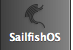
\includegraphics[scale=0.4]{../media/gfx/QtCreator/MerSDKsettings.png} 
  \caption{Choose ``SailfishOS'' from the left pane.}
  \label{fig:mersdkpkg:sailfishos}
\end{figure}
%
\subsubsection{zypper}\label{subsubsec:zypper}
%
Additional software and libraries come in \verb,RPM, packages and the management tool on the Mer SDK Build Engine is \verb,zypper,\footnote{As it was for the emulator before the Alpha3 SDK.}. It provides ``functions like repository access, dependency solving, package installation''\cite{suse01}.\\
\\
%
\begin{lstlisting}[language=bash]
[nemo@SailfishEmul ~]$ zypper refresh
\end{lstlisting}
will update the meta data that is stored from the package repository.
%
\\
\\
%
\begin{lstlisting}[language=bash]
[nemo@SailfishEmul ~]$ zypper search
\end{lstlisting}
will show you all packages that can be installed on the emulator.
%
\\
\\
\begin{lstlisting}[language=bash]
[nemo@SailfishEmul ~]$ zypper search boost
\end{lstlisting}
will show you all package names that contain \verb,boost,.
%
\\
\\
\begin{lstlisting}[language=bash]
[nemo@SailfishEmul ~]$ sudo zypper install boost-filesystem
\end{lstlisting}
will install the library \verb,boost-filesystem, and all its dependencies on the emulator. \emph{Note}: \verb,boost-filesystem, is not one of the currently available libraries\footnote{So why do I use it as an example? Honi soit qui mal y pense.}.
%
\\
\\
\begin{lstlisting}[language=bash]
[nemo@SailfishEmul ~]$ sudo zypper remove boost-filesystem
\end{lstlisting}
will remove the library \verb,boost-filesystem, and all its dependencies from the emulator.
Of course you can install additional software on the emulator\footnote{As long as this software is not part of your app.} that helps you to edit files directly or manage the filesystem better. 
%
\subsubsection{Known Logins}\label{subsubsec:mersdklogins}
%
\begin{tabular}{lll}
  \emph{user} & \emph{password} & \emph{comment} \\
  \hline 
  nemo & nemo & no private keys provided \\
  mersdk &  & for use with \verb,ssh, and private key \\
  root &  & no password needed in the VM \\
\end{tabular}
%
%
\subsubsection{SSH login}\label{subsubsec:mersdk:sshlogin}
%
Open your terminal and enter
%
\begin{lstlisting}[language=bash]
# connection as user mersdk
ssh -p 2222 -i ~/SailfishOS/vmshare/ssh/private_keys/engine/mersdk mersdk@localhost
-bash-3.2$ 
\end{lstlisting}
%
or
%
\begin{lstlisting}[language=bash]
# connection as user root
ssh -p 2222 -i /Users/sven/SailfishOS/vmshare/ssh/private_keys/engine/root root@localhost
Last login: Fri Dec  6 16:41:16 2013
[root@SailfishSDK ~]# 
\end{lstlisting}
%
%
\subsubsection{Public keys}
%
With the SDK come the public/private keys for SSH connections\footnote{There were some changes from Alpha1 to Alpha3 SDK.}.
%
\begin{lstlisting}[language=bash]
tree ~/SailfishOS/vmshare/ssh/private_keys 
/Users/sven/SailfishOS/vmshare/ssh/private_keys
+-- SailfishOS_Emulator
|   +-- nemo
|   +-- nemo.pub
|   +-- root
|   +-- root.pub
+-- engine
    +-- mersdk
    +-- mersdk.pub
    +-- root
    +-- root.pub
\end{lstlisting}
%